\documentclass[a4paper,10pt]{report}
\usepackage[utf8x]{inputenc}
\usepackage[T1]{fontenc}
\usepackage[a4paper]{geometry}
\usepackage[english]{babel}
\usepackage{graphicx}
\usepackage{listings}
\usepackage{fancybox}
\usepackage{xcolor}
\usepackage{pdfpages}
\usepackage{verbatim}


\title{ULB\\
        INFO-F403 - Introduction to language theory and compiling \\
            Introduction to language theory and compiling}
\author{\textsc{Bastogne} Jérôme,\\
        \textsc{Hereman} Nicolas}
\date{Academic year 2015-2016 - \today}

\begin{document}

\maketitle
\clearpage


\chapter{Part 2 - Grammar}

\section{The modified grammar}

This is our new modified grammar we ended up with : \\

\verbatiminput{../NewGrammar.txt}


\hfill \\
Removing unreachable and/or unproductive variables wasn't much of an issue but only a bit of work. The real deal in this part was to handle the correct associativity while removing left-recursion. Keeping the order of priority was not a problem. The problem is that we lost the associativity to the left when we tried to remove left-recursions. We tried multiple solutions to keep left associativity while removing left-recursions but none worked. So from here, we only could satisfy one of those constraints. We choosed to remove left-recursion because otherwise the algorithm wouldn't work. This means that our compiler works but is kind of false because left associativity is not respected.

\section{The action table}

To have the action table, we first needed to calculate the first and follow sets. Our grammar is LL(1), this means that LL(1) parsing uses only one symbol of input to predict the next grammar rule that should be used. Therefore each cell of our action table contains at most one rule.


\verbatiminput{../FirstAndFollow.txt}

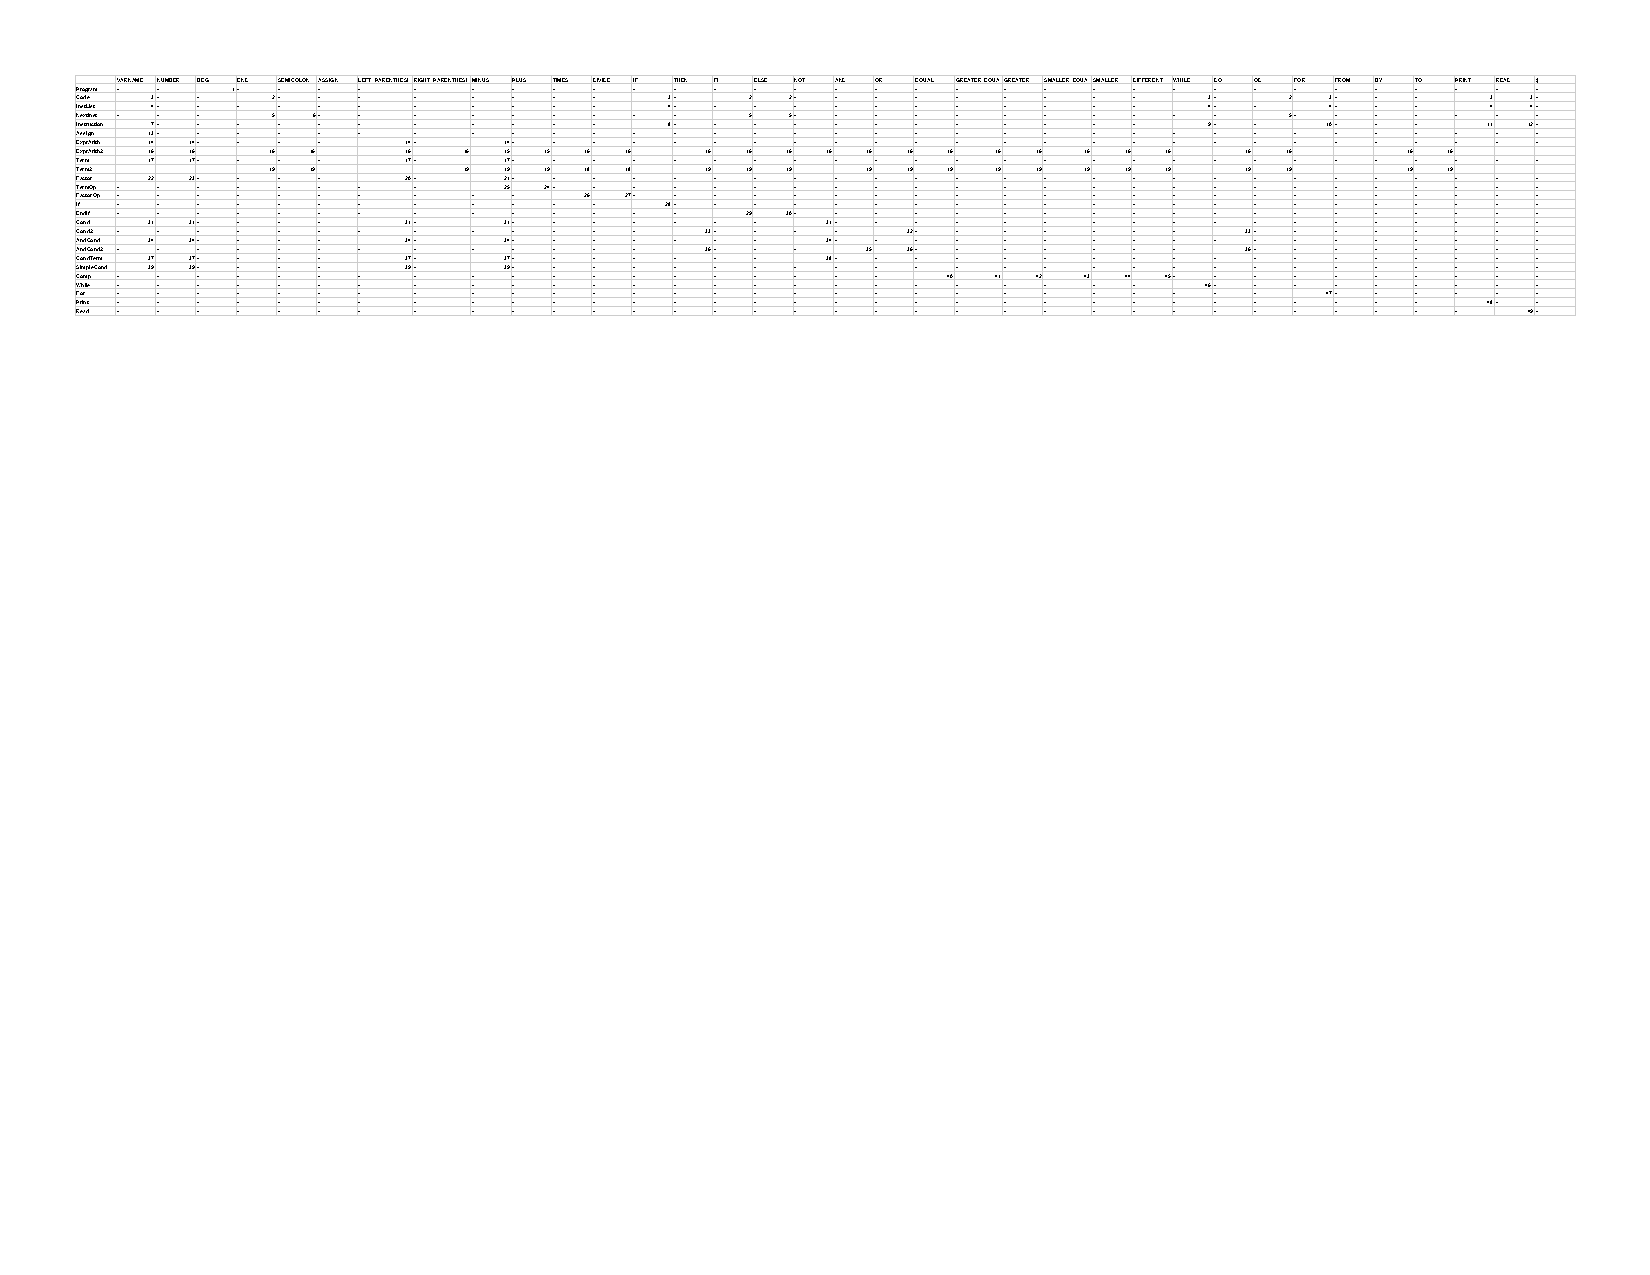
\includepdf[landscape=true]{TableauLL1.pdf}


\end{document}